
The ISE designs were evaluated using two different {\em host} cores:

\begin{itemize}
\item
    The \CORE{2} core\footnote{%
  \ifbool{anonymous}{Details of this core have been anonymised to comply with the TCHES submission guidelines.}{\href{https://github.com/scarv/scarv-cpu}}
}is a 5-stage, in-order scalar micro-controller.
    It implements the
    {\tt rv32imc}
    instruction set: 32-bit base ISA, with the Multiply and Compressed
    ISA extensions.
    A block diagram of the core is shown in~\REFFIG{fig:design:cpu_block:2}.
    The core has separate memory interfaces for instruction and data
    accesses, with no cache hierarchy or branch prediction.
    The core implements various performance counters,
    and
    elements of the
    RISC-V Privileged Resource Architecture 
    (PRA)~\cite[Chapter 3]{RV:ISA:II:17}
    related to exception and interrupt handling.

\item
    The \CORE{1} core\cite{rocket:16} 
    is a 5-stage, in-order pipeline with a configurable cache hierarchy and
    branch predictor.
    We used both 32-bit and 64-bit variants of \CORE{1} as bases for our work.
    We configured both base designs to have a single ``big" core, with
    no floating point support.
    ({\bf TODO:} List exactly how this configured Rocket)

\end{itemize}

Two modifications were made to the host cores to support the ISE variants:
1) The Instruction Decode module was modifed to support identification and
   operand selection for the new instructions. 
2) A new ``AES" functional unit (AES FU) was added to perform the instruction
   computations.
In the \CORE{2} core, the new block was built directly into the execution
pipeline.
For the \CORE{1}, we used the Rocket Custom Coprocessor (RoCC)
interface.
Because all of the ISE variants read at most two,
and write one general purpose register, no new structural datapaths
were needed.
This was an important design consideration, as RISC-V tries to
aggressivley follow this pattern.

All of the AES variants share the same sets of inputs, so the interface
to the AES FU is kept constant for every variant.
A synthesis time parameter was then added to switch between different
ISE variants for each host core.

The following sections give high level descriptions of the
instructions and their salient differences,
We list complete pseudo-code descriptions for each instruction
in the Appendix \REFSEC{sec:pseudo}.

\begin{figure}
\centering
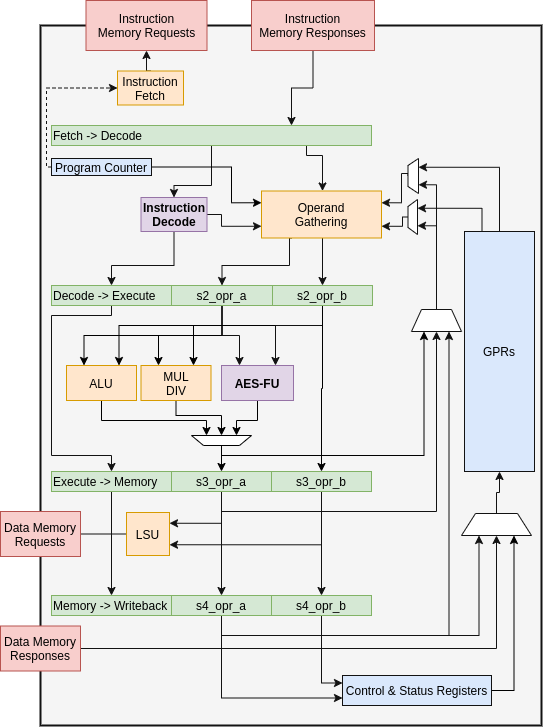
\includegraphics[scale=0.45,angle=90]{diagrams/scarv-cpu-uarch.png}
\caption{Core $2$: \CORE{2}.}
\label{fig:design:cpu_block:2}
\end{figure}

\begin{figure}
\centering
\begin{subfigure}[t]{0.40\textwidth}
    \centering
    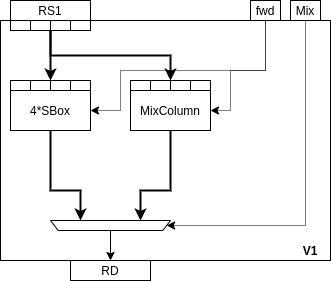
\includegraphics[width=\textwidth]{diagrams/ise-datapath-v1.png}
    \caption{Variant 1}
    \label{fig:design:fu_block:v1}
\end{subfigure}
\begin{subfigure}[t]{0.40\textwidth}
    \centering
    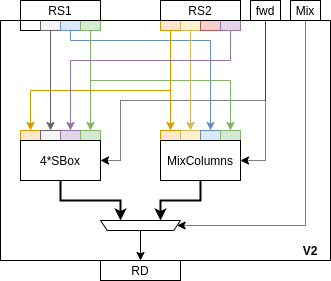
\includegraphics[width=\textwidth]{diagrams/ise-datapath-v2.png}
    \caption{Variant 2}
    \label{fig:design:fu_block:v2}
\end{subfigure}

\begin{subfigure}[t]{0.40\textwidth}
    \centering
    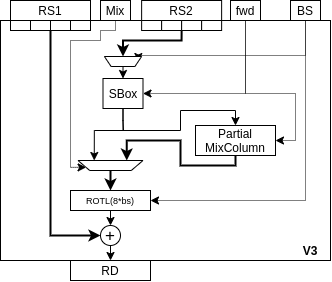
\includegraphics[width=\textwidth]{diagrams/ise-datapath-v3.png}
    \caption{Variant 3}
    \label{fig:design:fu_block:v3}
\end{subfigure}
\begin{subfigure}[t]{0.40\textwidth}
    \centering
    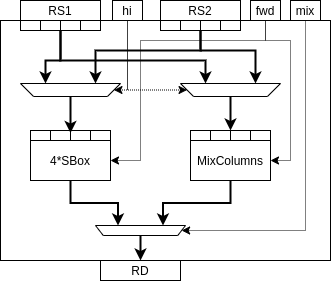
\includegraphics[width=\textwidth]{diagrams/ise-datapath-v5.png}
    \caption{Variant 5}
    \label{fig:design:fu_block:v5}
\end{subfigure}

\caption{
Micro-architecture block diagrams for the AES functional units, for
each ISE variant.
}
\end{figure}

